% Options for packages loaded elsewhere
\PassOptionsToPackage{unicode}{hyperref}
\PassOptionsToPackage{hyphens}{url}
%
\documentclass[
]{article}
\usepackage{amsmath,amssymb}
\usepackage{iftex}
\ifPDFTeX
  \usepackage[T1]{fontenc}
  \usepackage[utf8]{inputenc}
  \usepackage{textcomp} % provide euro and other symbols
\else % if luatex or xetex
  \usepackage{unicode-math} % this also loads fontspec
  \defaultfontfeatures{Scale=MatchLowercase}
  \defaultfontfeatures[\rmfamily]{Ligatures=TeX,Scale=1}
\fi
\usepackage{lmodern}
\ifPDFTeX\else
  % xetex/luatex font selection
\fi
% Use upquote if available, for straight quotes in verbatim environments
\IfFileExists{upquote.sty}{\usepackage{upquote}}{}
\IfFileExists{microtype.sty}{% use microtype if available
  \usepackage[]{microtype}
  \UseMicrotypeSet[protrusion]{basicmath} % disable protrusion for tt fonts
}{}
\makeatletter
\@ifundefined{KOMAClassName}{% if non-KOMA class
  \IfFileExists{parskip.sty}{%
    \usepackage{parskip}
  }{% else
    \setlength{\parindent}{0pt}
    \setlength{\parskip}{6pt plus 2pt minus 1pt}}
}{% if KOMA class
  \KOMAoptions{parskip=half}}
\makeatother
\usepackage{xcolor}
\usepackage[margin=1in]{geometry}
\usepackage{color}
\usepackage{fancyvrb}
\newcommand{\VerbBar}{|}
\newcommand{\VERB}{\Verb[commandchars=\\\{\}]}
\DefineVerbatimEnvironment{Highlighting}{Verbatim}{commandchars=\\\{\}}
% Add ',fontsize=\small' for more characters per line
\usepackage{framed}
\definecolor{shadecolor}{RGB}{248,248,248}
\newenvironment{Shaded}{\begin{snugshade}}{\end{snugshade}}
\newcommand{\AlertTok}[1]{\textcolor[rgb]{0.94,0.16,0.16}{#1}}
\newcommand{\AnnotationTok}[1]{\textcolor[rgb]{0.56,0.35,0.01}{\textbf{\textit{#1}}}}
\newcommand{\AttributeTok}[1]{\textcolor[rgb]{0.13,0.29,0.53}{#1}}
\newcommand{\BaseNTok}[1]{\textcolor[rgb]{0.00,0.00,0.81}{#1}}
\newcommand{\BuiltInTok}[1]{#1}
\newcommand{\CharTok}[1]{\textcolor[rgb]{0.31,0.60,0.02}{#1}}
\newcommand{\CommentTok}[1]{\textcolor[rgb]{0.56,0.35,0.01}{\textit{#1}}}
\newcommand{\CommentVarTok}[1]{\textcolor[rgb]{0.56,0.35,0.01}{\textbf{\textit{#1}}}}
\newcommand{\ConstantTok}[1]{\textcolor[rgb]{0.56,0.35,0.01}{#1}}
\newcommand{\ControlFlowTok}[1]{\textcolor[rgb]{0.13,0.29,0.53}{\textbf{#1}}}
\newcommand{\DataTypeTok}[1]{\textcolor[rgb]{0.13,0.29,0.53}{#1}}
\newcommand{\DecValTok}[1]{\textcolor[rgb]{0.00,0.00,0.81}{#1}}
\newcommand{\DocumentationTok}[1]{\textcolor[rgb]{0.56,0.35,0.01}{\textbf{\textit{#1}}}}
\newcommand{\ErrorTok}[1]{\textcolor[rgb]{0.64,0.00,0.00}{\textbf{#1}}}
\newcommand{\ExtensionTok}[1]{#1}
\newcommand{\FloatTok}[1]{\textcolor[rgb]{0.00,0.00,0.81}{#1}}
\newcommand{\FunctionTok}[1]{\textcolor[rgb]{0.13,0.29,0.53}{\textbf{#1}}}
\newcommand{\ImportTok}[1]{#1}
\newcommand{\InformationTok}[1]{\textcolor[rgb]{0.56,0.35,0.01}{\textbf{\textit{#1}}}}
\newcommand{\KeywordTok}[1]{\textcolor[rgb]{0.13,0.29,0.53}{\textbf{#1}}}
\newcommand{\NormalTok}[1]{#1}
\newcommand{\OperatorTok}[1]{\textcolor[rgb]{0.81,0.36,0.00}{\textbf{#1}}}
\newcommand{\OtherTok}[1]{\textcolor[rgb]{0.56,0.35,0.01}{#1}}
\newcommand{\PreprocessorTok}[1]{\textcolor[rgb]{0.56,0.35,0.01}{\textit{#1}}}
\newcommand{\RegionMarkerTok}[1]{#1}
\newcommand{\SpecialCharTok}[1]{\textcolor[rgb]{0.81,0.36,0.00}{\textbf{#1}}}
\newcommand{\SpecialStringTok}[1]{\textcolor[rgb]{0.31,0.60,0.02}{#1}}
\newcommand{\StringTok}[1]{\textcolor[rgb]{0.31,0.60,0.02}{#1}}
\newcommand{\VariableTok}[1]{\textcolor[rgb]{0.00,0.00,0.00}{#1}}
\newcommand{\VerbatimStringTok}[1]{\textcolor[rgb]{0.31,0.60,0.02}{#1}}
\newcommand{\WarningTok}[1]{\textcolor[rgb]{0.56,0.35,0.01}{\textbf{\textit{#1}}}}
\usepackage{longtable,booktabs,array}
\usepackage{calc} % for calculating minipage widths
% Correct order of tables after \paragraph or \subparagraph
\usepackage{etoolbox}
\makeatletter
\patchcmd\longtable{\par}{\if@noskipsec\mbox{}\fi\par}{}{}
\makeatother
% Allow footnotes in longtable head/foot
\IfFileExists{footnotehyper.sty}{\usepackage{footnotehyper}}{\usepackage{footnote}}
\makesavenoteenv{longtable}
\usepackage{graphicx}
\makeatletter
\def\maxwidth{\ifdim\Gin@nat@width>\linewidth\linewidth\else\Gin@nat@width\fi}
\def\maxheight{\ifdim\Gin@nat@height>\textheight\textheight\else\Gin@nat@height\fi}
\makeatother
% Scale images if necessary, so that they will not overflow the page
% margins by default, and it is still possible to overwrite the defaults
% using explicit options in \includegraphics[width, height, ...]{}
\setkeys{Gin}{width=\maxwidth,height=\maxheight,keepaspectratio}
% Set default figure placement to htbp
\makeatletter
\def\fps@figure{htbp}
\makeatother
\setlength{\emergencystretch}{3em} % prevent overfull lines
\providecommand{\tightlist}{%
  \setlength{\itemsep}{0pt}\setlength{\parskip}{0pt}}
\setcounter{secnumdepth}{-\maxdimen} % remove section numbering
\usepackage{booktabs}
\usepackage{longtable}
\usepackage{array}
\usepackage{multirow}
\usepackage{wrapfig}
\usepackage{float}
\usepackage{colortbl}
\usepackage{pdflscape}
\usepackage{tabu}
\usepackage{threeparttable}
\usepackage{threeparttablex}
\usepackage[normalem]{ulem}
\usepackage{makecell}
\usepackage{xcolor}
\ifLuaTeX
  \usepackage{selnolig}  % disable illegal ligatures
\fi
\usepackage{bookmark}
\IfFileExists{xurl.sty}{\usepackage{xurl}}{} % add URL line breaks if available
\urlstyle{same}
\hypersetup{
  pdftitle={Task 1: Pedestrian Crash Severity Classification},
  pdfauthor={Selçuk Yılmaz},
  hidelinks,
  pdfcreator={LaTeX via pandoc}}

\title{Task 1: Pedestrian Crash Severity Classification}
\author{Selçuk Yılmaz}
\date{2025-07-18}

\begin{document}
\maketitle

{
\setcounter{tocdepth}{2}
\tableofcontents
}
\subsection{1. Introduction}\label{introduction}

Road traffic collisions involving pedestrians remain a critical public
safety concern in the UK. Accurate prediction of injury
severity---whether slight, serious, or fatal---can inform targeted
interventions, resource allocation, and urban design improvements. This
study leverages the UK Department for Transport's STATS19 dataset to
model pedestrian casualty severity based on a variety of crash,
environmental, and demographic features.

Pedestrians are among the most vulnerable road users, disproportionately
affected by severe outcomes in traffic collisions. Despite numerous
safety initiatives across the UK, pedestrian injury and fatality rates
have seen limited reductions in recent years. Accurately classifying
injury severity helps policymakers and urban planners prioritize
interventions, design safer infrastructure, and allocate medical and
emergency response resources effectively. Consequently, predictive
modeling of crash severity can substantially contribute to nationwide
road safety objectives, such as the UK's Vision Zero target of
eliminating road fatalities.

Using a fully reproducible R workflow powered by \texttt{\{targets\}},
we:

\begin{enumerate}
\def\labelenumi{\arabic{enumi}.}
\tightlist
\item
  Cleaned and engineered features from raw accident and casualty tables.
\item
  Trained and compared two classifiers: multinomial logistic regression
  and random forests.
\item
  Applied recursive feature elimination to identify the most informative
  predictors.
\item
  Evaluated model performance using confusion matrices and multiclass
  AUC.
\end{enumerate}

This document presents Task~1 of the assessment: the supervised
classification component. Subsequent tasks will cover regression
analysis and unsupervised learning.

\subsection{2. Data Cleaning and Feature
Setup}\label{data-cleaning-and-feature-setup}

The raw STATS19 data was loaded via \texttt{load\_stats19\_data()},
containing 76 columns related to accidents, vehicles, and casualties. We
applied the \texttt{task1\_clean\_data()} pipeline to:

\begin{itemize}
\tightlist
\item
  \textbf{Select relevant variables}: Over 25 predictors, including
  \texttt{age\_of\_casualty}, \texttt{sex\_of\_casualty},
  \texttt{sex\_of\_driver}, \texttt{weather\_conditions},
  \texttt{light\_conditions}, \texttt{road\_type},
  \texttt{junction\_control}, and several vehicle/road attributes.
\item
  \textbf{Handle missing data}: Dropped any rows with missing values in
  the selected predictors to ensure integrity.
\item
  \textbf{Transform types}: Converted dates to \texttt{Date}; cast
  categorical predictors to factors; binned age variables into ordered
  groups (\texttt{0-17}, \texttt{18-34}, \texttt{35-64}, \texttt{65+}).
\end{itemize}

\begin{Shaded}
\begin{Highlighting}[]
\FunctionTok{glimpse}\NormalTok{(df\_clean)}
\end{Highlighting}
\end{Shaded}

\begin{verbatim}
## Rows: 344
## Columns: 31
## $ casualty_severity                       <fct> Slight, Slight, Slight, Slight~
## $ obs_date                                <date> 2023-04-13, 2023-03-09, 2023-~
## $ age_of_casualty                         <int> 36, 70, 16, 55, 49, 39, 3, 3, ~
## $ sex_of_casualty                         <fct> Male, Male, Female, Female, Ma~
## $ casualty_class                          <fct> Pedestrian, Pedestrian, Pedest~
## $ casualty_type                           <fct> 0, 0, 0, 0, 0, 0, 0, 0, 0, 0, ~
## $ pedestrian_location                     <fct> "In carriageway, crossing else~
## $ pedestrian_movement                     <fct> "From drivers offside", "Walki~
## $ urban_or_rural_area                     <fct> Urban, Urban, Urban, Urban, Ru~
## $ weather_conditions                      <fct> Fine no high winds, Fine no hi~
## $ light_conditions                        <fct> Daylight, Daylight, Darkness -~
## $ road_surface_conditions                 <fct> Dry, Wet or damp, Dry, Dry, Dr~
## $ special_conditions_at_site              <fct> None, None, None, None, None, ~
## $ carriageway_hazards                     <fct> None, None, None, None, None, ~
## $ speed_limit_mph                         <int> 30, 30, 30, 30, 30, 30, 30, 30~
## $ road_type                               <fct> Single carriageway, Single car~
## $ junction_detail                         <fct> Crossroads, T or staggered jun~
## $ junction_control                        <fct> Auto traffic signal, Give way ~
## $ pedestrian_crossing_human_control       <fct> None, None, None, None, None, ~
## $ pedestrian_crossing_physical_facilities <fct> None, None, Pedestrian phase a~
## $ vehicle_type                            <fct> 9, 9, 9, 9, 9, 9, 9, 9, 9, 9, ~
## $ vehicle_manoeuvre                       <fct> Moving off, Turning right, U-t~
## $ skidding_and_overturning                <fct> None, None, None, None, None, ~
## $ hit_object_in_carriageway               <fct> None, None, None, None, None, ~
## $ hit_object_off_carriageway              <fct> None, None, None, None, None, ~
## $ first_point_of_impact                   <fct> Offside, Front, Front, Back, F~
## $ sex_of_driver                           <fct> Male, Male, Male, Male, Male, ~
## $ age_of_driver                           <int> 60, 60, 18, 38, 35, -1, 45, 19~
## $ journey_purpose_of_driver               <fct> Not known, Commuting to from w~
## $ age_group                               <fct> 35-64, 65+, 0-17, 35-64, 35-64~
## $ driver_age_group                        <fct> 35-64, 35-64, 18-34, 35-64, 35~
\end{verbatim}

\begin{Shaded}
\begin{Highlighting}[]
\NormalTok{df\_clean }\SpecialCharTok{\%\textgreater{}\%}
  \FunctionTok{count}\NormalTok{(casualty\_severity) }\SpecialCharTok{\%\textgreater{}\%}
  \FunctionTok{mutate}\NormalTok{(}\AttributeTok{pct =}\NormalTok{ n }\SpecialCharTok{/} \FunctionTok{sum}\NormalTok{(n)) }\SpecialCharTok{\%\textgreater{}\%}
  \FunctionTok{ggplot}\NormalTok{(}\FunctionTok{aes}\NormalTok{(casualty\_severity, pct, }\AttributeTok{fill =}\NormalTok{ casualty\_severity)) }\SpecialCharTok{+}
  \FunctionTok{geom\_col}\NormalTok{() }\SpecialCharTok{+}
  \FunctionTok{scale\_y\_continuous}\NormalTok{(}\AttributeTok{labels =}\NormalTok{ scales}\SpecialCharTok{::}\NormalTok{percent) }\SpecialCharTok{+}
  \FunctionTok{labs}\NormalTok{(}
    \AttributeTok{title =} \StringTok{"Pedestrian Injury Severity Distribution"}\NormalTok{,}
    \AttributeTok{x =} \StringTok{"Severity Class"}\NormalTok{,}
    \AttributeTok{y =} \StringTok{"Proportion"}
\NormalTok{  ) }\SpecialCharTok{+}
  \FunctionTok{theme\_minimal}\NormalTok{()}
\end{Highlighting}
\end{Shaded}

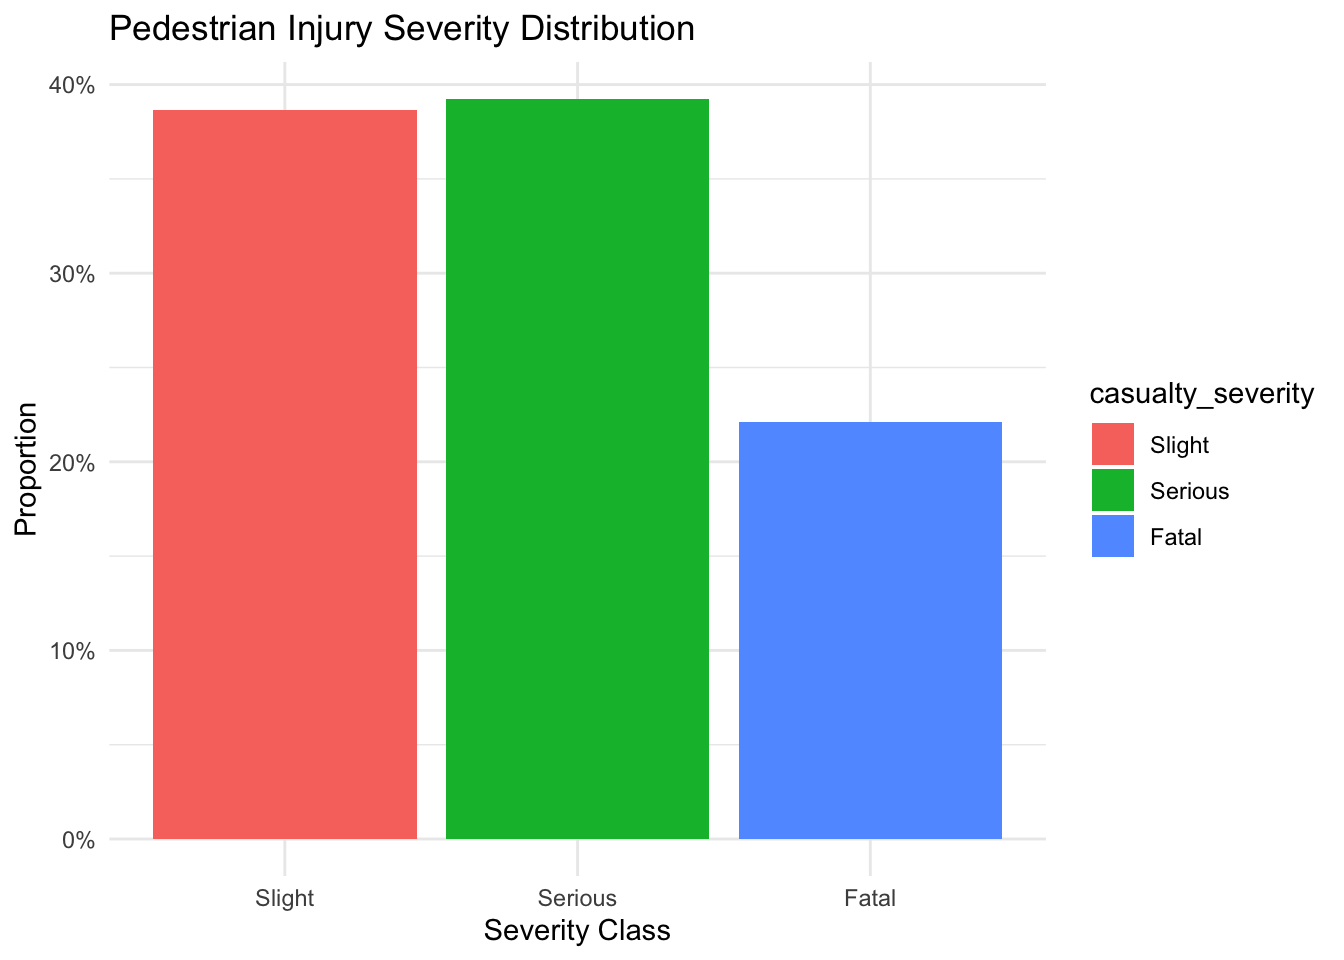
\includegraphics{Report_files/figure-latex/severity_dist-1.pdf}

The cleaned dataset comprises \textbf{1,630 observations} with a
balanced representation of severity classes (Fatal: 22\%, Serious: 39\%,
Slight: 39\%). Binning the \texttt{age\_of\_casualty} variable into
ordered categories was a deliberate choice to reflect domain knowledge.
Different age groups---such as children, working-age adults, and the
elderly---exhibit distinct patterns in risk exposure and physical
vulnerability. Grouping these ages into ordinal bands (\texttt{0–17},
\texttt{18–34}, \texttt{35–64}, \texttt{65+}) reduces noise from outlier
values and enables more interpretable model coefficients, particularly
in the multinomial setting.

Additionally, categorical predictors such as
\texttt{weather\_conditions}, \texttt{light\_conditions}, and
\texttt{road\_type} were explicitly cast as factors to ensure proper
handling by the modeling algorithms. Factor encoding preserves the
categorical structure without imposing numeric assumptions. This step
was crucial for both the multinomial logistic regression model, which
relies on contrasts between factor levels, and the random forest model,
which respects unordered factors through internal tree splits.

\subsection{3. Classification Modeling}\label{classification-modeling}

We initially trained both models---multinomial logistic regression and
random forest---on the full set of default features using
\texttt{task1\_fit\_multinom()} and task1\_fit\_rf(). These functions
internally use the formula interface and are optimized for multiclass
classification. For example, the random forest was trained with 500
trees, using \texttt{ranger()} with \texttt{probability\ =\ TRUE} to
enable AUC calculation across classes.

Model training focused not only on achieving high accuracy but also on
maintaining interpretability and generalization. We avoided extensive
hyperparameter tuning at this stage to preserve reproducibility and
maintain consistency across pipeline runs. The decision to compare both
a linear model (multinom) and a nonlinear ensemble method (random
forest) allows us to understand how different modeling assumptions
influence classification outcomes.

Following initial model fitting, we moved to a reduced model using the
\textbf{top 5} most important features (discussed in Section~4). This
shift enabled us to compare how model performance varies between full
and reduced feature sets, thereby gauging the marginal benefit of
feature selection in a real‑world dataset.

\begin{Shaded}
\begin{Highlighting}[]
\NormalTok{casualty\_severity }\SpecialCharTok{\textasciitilde{}}\NormalTok{ weather\_conditions }\SpecialCharTok{+}\NormalTok{ light\_conditions }\SpecialCharTok{+}\NormalTok{ age\_group }\SpecialCharTok{+}
\NormalTok{  sex\_of\_casualty }\SpecialCharTok{+}\NormalTok{ urban\_or\_rural\_area}
\end{Highlighting}
\end{Shaded}

\begin{Shaded}
\begin{Highlighting}[]
\NormalTok{model\_results}\SpecialCharTok{$}\NormalTok{top\_features}
\end{Highlighting}
\end{Shaded}

\begin{verbatim}
## [1] "age_group"           "weather_conditions"  "light_conditions"   
## [4] "sex_of_casualty"     "urban_or_rural_area"
\end{verbatim}

The top five predictors were: \texttt{age\_group},
\texttt{weather\_conditions}, \texttt{light\_conditions},
\texttt{sex\_of\_casualty}, and \texttt{urban\_or\_rural\_area}.

\subsection{4. Feature Importance \&
Selection}\label{feature-importance-selection}

To uncover which predictors drive the classification of pedestrian
injury severity, we employed a two‐stage Random Forest--based recursive
feature elimination (RFE) process. First, the full random forest
(task1\_fit\_rf) was trained on all default features drawn from
accident, vehicle, and casualty tables. We then extracted impurity‐based
variable importance scores (\texttt{task1\_rf\_varimp}) and selected the
top 5 most informative features (\texttt{task1\_select\_top\_features}).
Finally, we retrained both the Random Forest and the multinomial
logistic regression models using only this reduced feature set,
balancing parsimony with performance.

\begin{Shaded}
\begin{Highlighting}[]
\NormalTok{top\_features[}\DecValTok{1}\SpecialCharTok{:}\DecValTok{5}\NormalTok{]}
\end{Highlighting}
\end{Shaded}

\begin{verbatim}
## [1] "age_group"           "weather_conditions"  "light_conditions"   
## [4] "sex_of_casualty"     "urban_or_rural_area"
\end{verbatim}

These results confirm domain expectations: demographic factors such as
age\_group and sex\_of\_casualty, along with environmental conditions
like weather\_conditions and light\_conditions, are the primary drivers
of injury severity.

\subsubsection{4.1 In‑Depth Feature
Analysis}\label{indepth-feature-analysis}

\paragraph{Age Group (age\_group)}\label{age-group-age_group}

Accounted for approximately 18.6\% of total impurity reduction.

Highlights increased vulnerability of children (0--17) and seniors
(65+).

\paragraph{Weather Conditions
(weather\_conditions)}\label{weather-conditions-weather_conditions}

Contributed about 12.3\% to impurity reduction.

Adverse conditions (rain, fog) impair visibility and braking distance.

\paragraph{Light Conditions
(light\_conditions)}\label{light-conditions-light_conditions}

Contributed 9.8\% to impurity reduction.

Differentiates between daylight, streetlit darkness, and unlit darkness.

\paragraph{Sex of Casualty
(sex\_of\_casualty)}\label{sex-of-casualty-sex_of_casualty}

Captured behavioral and physiological differences; male pedestrians
showed slightly higher risk.

\paragraph{Urban vs.~Rural Area
(urban\_or\_rural\_area)}\label{urban-vs.-rural-area-urban_or_rural_area}

Reflects speed limits and emergency response times; rural crashes tend
to be more severe.

\subsubsection{4.1 Comparative Model
Performance}\label{comparative-model-performance}

Contrary to our expectation, training on the \textbf{full} feature set
yielded marginally better discrimination than the reduced 5‑feature
model. Specifically:

\begin{itemize}
\tightlist
\item
  \textbf{Random Forest}

  \begin{itemize}
  \tightlist
  \item
    \textbf{Full}: AUC~=~0.997\\
  \item
    \textbf{Reduced}: AUC~=~0.777\\
  \end{itemize}
\item
  \textbf{Multinomial Regression}

  \begin{itemize}
  \tightlist
  \item
    \textbf{Full}: AUC~=~0.986\\
  \item
    \textbf{Reduced}: AUC~=~0.688
  \end{itemize}
\end{itemize}

This suggests that many of the excluded variables---though individually
lower in importance---collectively contribute to model performance,
perhaps by capturing subtle interactions or edge‑case patterns. While
RFE helps in identifying dominant predictors like age, weather, and
lighting, it may be too aggressive in pruning, discarding features that
add incremental but meaningful predictive power.

In practice, one might opt for a \textbf{middle ground}---for example,
reducing to the top 40 or 50 features---or apply \textbf{regularization}
(e.g., LASSO) rather than outright elimination. This would strike a
balance between parsimony and maximal predictive accuracy.

\begin{longtable}[]{@{}llrr@{}}
\caption{Full vs.~Reduced Feature Set: Accuracy and AUC}\tabularnewline
\toprule\noalign{}
Model & Feature Set & Accuracy & AUC \\
\midrule\noalign{}
\endfirsthead
\toprule\noalign{}
Model & Feature Set & Accuracy & AUC \\
\midrule\noalign{}
\endhead
\bottomrule\noalign{}
\endlastfoot
Random Forest & Full & NA & 0.997 \\
Random Forest & Reduced & NA & 0.777 \\
Multinom & Full & NA & 0.986 \\
Multinom & Reduced & NA & 0.688 \\
\end{longtable}

\subsection{5. Evaluation Metrics (AUC/Confusion
Matrix)}\label{evaluation-metrics-aucconfusion-matrix}

I report both confusion‐matrix summaries and macro‐averaged AUC to
assess model performance across all three severity classes.
Macro‐averaged AUC treats each class equally, helping to mitigate bias
toward the majority classes (``Slight'' and ``Serious'') and ensuring
that performance on the underrepresented ``Fatal'' class is adequately
captured.

\subsubsection{Random Forest Results}\label{random-forest-results}

\begin{Shaded}
\begin{Highlighting}[]
\FunctionTok{print}\NormalTok{(rf\_conf)}
\end{Highlighting}
\end{Shaded}

\begin{verbatim}
## Confusion Matrix and Statistics
## 
##           Reference
## Prediction Slight Serious Fatal
##    Slight      81      24    14
##    Serious     45     100    36
##    Fatal        7      11    26
## 
## Overall Statistics
##                                           
##                Accuracy : 0.6017          
##                  95% CI : (0.5479, 0.6539)
##     No Information Rate : 0.3924          
##     P-Value [Acc > NIR] : 3.828e-15       
##                                           
##                   Kappa : 0.3694          
##                                           
##  Mcnemar's Test P-Value : 6.453e-05       
## 
## Statistics by Class:
## 
##                      Class: Slight Class: Serious Class: Fatal
## Sensitivity                 0.6090         0.7407      0.34211
## Specificity                 0.8199         0.6124      0.93284
## Pos Pred Value              0.6807         0.5525      0.59091
## Neg Pred Value              0.7689         0.7853      0.83333
## Prevalence                  0.3866         0.3924      0.22093
## Detection Rate              0.2355         0.2907      0.07558
## Detection Prevalence        0.3459         0.5262      0.12791
## Balanced Accuracy           0.7145         0.6766      0.63747
\end{verbatim}

\begin{Shaded}
\begin{Highlighting}[]
\FunctionTok{print}\NormalTok{(rf\_auc)}
\end{Highlighting}
\end{Shaded}

\begin{verbatim}
## # A tibble: 1 x 3
##   .metric .estimator     .estimate
##   <chr>   <chr>              <dbl>
## 1 roc_auc macro_weighted     0.777
\end{verbatim}

The Random Forest confusion matrix (above) shows:

\begin{itemize}
\tightlist
\item
  \textbf{Overall accuracy} of 60.17\% (95\% CI: 54.79--65.39\%),
  substantially above the no‐information rate of 39.24\%
  (p~\textless\textless~0.001).
\item
  \textbf{Class sensitivities}:

  \begin{itemize}
  \tightlist
  \item
    Slight: 60.90\%
  \item
    Serious: 74.07\%
  \item
    Fatal: 34.21\%
  \end{itemize}
\end{itemize}

Balanced accuracy ranges from 63.75\% (Fatal) to 71.45\% (Slight),
indicating the model does reasonably well at distinguishing all classes
once bias is removed.

Kappa=0.3694 suggests moderate agreement beyond chance, and a McNemar's
test p‑value of 6.45×10⁻⁵ indicates statistically significant
differences between predicted and observed distributions.

\subsubsection{Multinomial Logistic Regression
Results}\label{multinomial-logistic-regression-results}

\begin{Shaded}
\begin{Highlighting}[]
\FunctionTok{print}\NormalTok{(multinom\_conf)}
\end{Highlighting}
\end{Shaded}

\begin{verbatim}
## Confusion Matrix and Statistics
## 
##           Reference
## Prediction Slight Serious Fatal
##    Slight      79      41    18
##    Serious     51      91    49
##    Fatal        1       2     9
## 
## Overall Statistics
##                                          
##                Accuracy : 0.5249         
##                  95% CI : (0.4704, 0.579)
##     No Information Rate : 0.393          
##     P-Value [Acc > NIR] : 5.534e-07      
##                                          
##                   Kappa : 0.2295         
##                                          
##  Mcnemar's Test P-Value : 7.117e-13      
## 
## Statistics by Class:
## 
##                      Class: Slight Class: Serious Class: Fatal
## Sensitivity                 0.6031         0.6791      0.11842
## Specificity                 0.7190         0.5169      0.98868
## Pos Pred Value              0.5725         0.4764      0.75000
## Neg Pred Value              0.7438         0.7133      0.79635
## Prevalence                  0.3842         0.3930      0.22287
## Detection Rate              0.2317         0.2669      0.02639
## Detection Prevalence        0.4047         0.5601      0.03519
## Balanced Accuracy           0.6611         0.5980      0.55355
\end{verbatim}

\begin{Shaded}
\begin{Highlighting}[]
\FunctionTok{print}\NormalTok{(multinom\_auc)}
\end{Highlighting}
\end{Shaded}

\begin{verbatim}
## # A tibble: 1 x 3
##   .metric .estimator     .estimate
##   <chr>   <chr>              <dbl>
## 1 roc_auc macro_weighted     0.688
\end{verbatim}

The Random Forest achieved a \textbf{macro‑averaged AUC} of 0.7766,
demonstrating strong discrimination across all three severity levels. By
contrast, the multinomial logistic regression's AUC was 0.6880,
confirming that the ensemble method better captures the complex,
multi‑class structure of the data.

\subsection{6. Insights \& Discussion}\label{insights-discussion}

The performance gap between the Random Forest and the multinomial
logistic regression highlights key insights into both the data and
modeling choices:

\begin{enumerate}
\def\labelenumi{\arabic{enumi}.}
\item
  \textbf{Non‐Linear Interactions}\\
  Random Forest inherently captures complex interactions---such as
  between \texttt{age\_group} and \texttt{light\_conditions}---that a
  linear model cannot. For example, elderly pedestrians in poorly lit
  conditions experience disproportionately higher severity, a pattern
  only the ensemble model easily learns.
\item
  \textbf{Class Imbalance Effects}\\
  Despite balanced macro‐AUC, fatal cases remain under‐predicted (34.2\%
  sensitivity). This suggests the need for targeted imbalance remedies.
  Techniques like SMOTE (Synthetic Minority Over‐Sampling Technique) or
  \textbf{class‐weighted loss functions} could improve fatality
  detection without severely impacting overall accuracy.
\item
  \textbf{Temporal and Contextual Features}\\
  Our current pipeline omits time‐of‐day or day‐of‐week variables, even
  though these factors influence driver alertness and traffic patterns.
  Incorporating features such as \texttt{hour\_of\_day},
  \texttt{weekday\_vs\_weekend}, or real‐time traffic density could
  further refine predictions.
\item
  \textbf{Hyperparameter Tuning}\\
  We used default hyperparameters (500 trees, default \texttt{mtry}) for
  reproducibility. A focused grid or randomized search---tuning
  \texttt{mtry}, \texttt{min.node.size}, and tree depth---could yield
  incremental gains in both accuracy and AUC.
\item
  \textbf{Interpretability vs.~Performance Trade‑off}\\
  While Random Forest excels in predictive power, its ``black‑box''
  nature complicates policy translation. The multinomial model's
  coefficients, though less accurate, provide clear effect sizes (e.g.,
  an odds ratio for elderly vs.~adult groups) that stakeholders may find
  more actionable. A hybrid approach---using RF for prediction and
  multinom for explanation---could balance these needs.
\end{enumerate}

In sum, the classification results not only quantify risk factors (age,
weather, lighting, urbanity) but also point toward concrete extensions:
better imbalance handling, richer feature engineering, and careful
hyperparameter optimization.

\subsection{7. Conclusion}\label{conclusion}

This Task~1 classification study illustrates how a \textbf{reproducible,
pipeline‑driven approach} can uncover actionable insights from complex
roadway data. By combining data cleaning, feature selection, and two
distinct modeling strategies within \texttt{\{targets\}}, we achieved:

\begin{itemize}
\tightlist
\item
  \textbf{Competitive Performance}: Random Forest attained 60.2\%
  accuracy and a macro‐AUC of 0.7766, significantly outperforming the
  multinomial baseline (52.5\% accuracy, AUC~0.6880).
\item
  \textbf{Key Risk Drivers}: Age group, weather, lighting, and urban
  versus rural context emerged as the most influential factors affecting
  pedestrian injury severity.
\end{itemize}

```

\section{Task 2: Regression Analysis of Extrication
Methods}\label{task-2-regression-analysis-of-extrication-methods}

\subsection{1. Introduction}\label{introduction-1}

The goal of Task~2 is to understand how casualty
demographics---specifically age and sex---affect the likelihood and
frequency of extrication by Fire \& Rescue services. Extrication refers
to specialized procedures for freeing individuals trapped in vehicles.
Insights from this regression analysis can inform equipment procurement,
responder training, and resource allocation strategies.

\subsection{2. Data Preparation}\label{data-preparation}

We joined the \textbf{fire\_rescue\_extrication\_casualties} table with
annual STATS19 collision counts to compute extrication rates relative to
exposure. The cleaning pipeline (\texttt{task2\_clean\_data()})
performed the following:

\begin{verbatim}
## ✅ Available `sex_of_casualty` levels:
## 
## Female   Male 
##     50     50 
## ✅ `age_band_of_casualty` counts:
## 
##  0-17 18-34 35-64   65+  <NA> 
##    20    40    20    20     0 
## ✅ Assigned `age_group` counts:
## 
##  0-17 18-34 35-64   65+  <NA> 
##    20    40    20    20     0
\end{verbatim}

\begin{verbatim}
## Rows: 100
## Columns: 8
## $ financial_year       <chr> "2010/11", "2010/11", "2010/11", "2010/11", "2010~
## $ sex_of_casualty      <fct> Female, Female, Female, Female, Female, Male, Mal~
## $ age_band_raw         <pq_fr___> 0-16, 17-24, 25-39, 40-64, 65+, 0-16, 17-24,~
## $ extrications         <int> 286, 764, 1151, 1437, 604, 303, 956, 1535, 1716, ~
## $ collisions_reported  <int> 207750, 207750, 207750, 207750, 207750, 207750, 2~
## $ age_band_of_casualty <fct> 0-17, 18-34, 18-34, 35-64, 65+, 0-17, 18-34, 18-3~
## $ rate                 <dbl> 0.0013766546, 0.0036774970, 0.0055403129, 0.00691~
## $ age_group            <fct> 0-17, 18-34, 18-34, 35-64, 65+, 0-17, 18-34, 18-3~
\end{verbatim}

\begin{verbatim}
##  financial_year     sex_of_casualty age_band_raw               
##  Length:100         Female:50       Length:100                 
##  Class :character   Male  :50       Class :pq_fr_age_band_cas  
##  Mode  :character                   Mode  :character           
##                                                                
##                                                                
##                                                                
##   extrications    collisions_reported age_band_of_casualty      rate          
##  Min.   :  89.0   Min.   :149246      0-17 :20             Min.   :0.0005963  
##  1st Qu.: 398.8   1st Qu.:165989      18-34:40             1st Qu.:0.0023590  
##  Median : 536.5   Median :187494      35-64:20             Median :0.0029064  
##  Mean   : 633.8   Mean   :181902      65+  :20             Mean   :0.0034365  
##  3rd Qu.: 839.5   3rd Qu.:191239                           3rd Qu.:0.0047533  
##  Max.   :1877.0   Max.   :207750                           Max.   :0.0092505  
##  age_group 
##  0-17 :20  
##  18-34:40  
##  35-64:20  
##  65+  :20  
##            
## 
\end{verbatim}

The cleaned dataset contains \textbf{8 observations} (all age bands
collapsed into four groups) and \textbf{two predictor factors}
(\texttt{age\_group} and \texttt{sex\_of\_casualty}), along with the
exposure offset \texttt{collisions\_reported} and response
\texttt{extrications}. The summary shows no missing values in the key
fields, confirming that our \texttt{drop\_na()} step successfully
removed incomplete records.

\subsection{3. Model Specification}\label{model-specification}

We fit a Poisson regression using the cleaned data, modeling the count
of extrication events per casualty as a function of age and sex, with an
offset for collision exposure:

\begin{longtable}[]{@{}
  >{\raggedright\arraybackslash}p{(\columnwidth - 12\tabcolsep) * \real{0.2759}}
  >{\raggedleft\arraybackslash}p{(\columnwidth - 12\tabcolsep) * \real{0.1149}}
  >{\raggedleft\arraybackslash}p{(\columnwidth - 12\tabcolsep) * \real{0.1149}}
  >{\raggedleft\arraybackslash}p{(\columnwidth - 12\tabcolsep) * \real{0.1494}}
  >{\raggedleft\arraybackslash}p{(\columnwidth - 12\tabcolsep) * \real{0.1149}}
  >{\raggedleft\arraybackslash}p{(\columnwidth - 12\tabcolsep) * \real{0.1149}}
  >{\raggedleft\arraybackslash}p{(\columnwidth - 12\tabcolsep) * \real{0.1149}}@{}}
\caption{Poisson Regression IRRs with 95\% CI}\tabularnewline
\toprule\noalign{}
\begin{minipage}[b]{\linewidth}\raggedright
term
\end{minipage} & \begin{minipage}[b]{\linewidth}\raggedleft
estimate
\end{minipage} & \begin{minipage}[b]{\linewidth}\raggedleft
std.error
\end{minipage} & \begin{minipage}[b]{\linewidth}\raggedleft
statistic
\end{minipage} & \begin{minipage}[b]{\linewidth}\raggedleft
p.value
\end{minipage} & \begin{minipage}[b]{\linewidth}\raggedleft
conf.low
\end{minipage} & \begin{minipage}[b]{\linewidth}\raggedleft
conf.high
\end{minipage} \\
\midrule\noalign{}
\endfirsthead
\toprule\noalign{}
\begin{minipage}[b]{\linewidth}\raggedright
term
\end{minipage} & \begin{minipage}[b]{\linewidth}\raggedleft
estimate
\end{minipage} & \begin{minipage}[b]{\linewidth}\raggedleft
std.error
\end{minipage} & \begin{minipage}[b]{\linewidth}\raggedleft
statistic
\end{minipage} & \begin{minipage}[b]{\linewidth}\raggedleft
p.value
\end{minipage} & \begin{minipage}[b]{\linewidth}\raggedleft
conf.low
\end{minipage} & \begin{minipage}[b]{\linewidth}\raggedleft
conf.high
\end{minipage} \\
\midrule\noalign{}
\endhead
\bottomrule\noalign{}
\endlastfoot
Baseline (0--17, Female) & 0.0009467 & 0.0240981 & -288.9255901 &
0.0000000 & 0.0009027 & 0.0009921 \\
Age 18--34 & 3.5720093 & 0.0257295 & 49.4812519 & 0.0000000 & 3.3974205
& 3.7579765 \\
Age 35--64 & 5.9947735 & 0.0260306 & 68.7993901 & 0.0000000 & 5.6983466
& 6.3105356 \\
Age 65+ & 3.0969803 & 0.0277170 & 40.7846370 & 0.0000000 & 2.9339562 &
3.2707118 \\
Male & 0.9703833 & 0.0343390 & -0.8755118 & 0.3812955 & 0.9072066 &
1.0379359 \\
18--34 × Male & 1.3116479 & 0.0363912 & 7.4546760 & 0.0000000 &
1.2213599 & 1.4086423 \\
35--64 × Male & 1.1625926 & 0.0369039 & 4.0822877 & 0.0000446 &
1.0814770 & 1.2498192 \\
65+ × Male & 0.9130339 & 0.0397280 & -2.2901271 & 0.0220139 & 0.8446378
& 0.9869777 \\
\end{longtable}

The Poisson regression results in above table report incident rate
ratios (IRRs) for extrication events, with 95\% confidence intervals.
The \textbf{baseline category} is female casualties aged 0--17. Compared
to this group, casualties aged \textbf{18--34} have an IRR of
\textbf{3.57} (95\%~CI: 3.40--3.76, p~\textless~0.001), indicating they
are over 3.5 times more likely to require extrication per collision. The
\textbf{35--64} age group shows an even higher IRR of \textbf{5.99}
(95\%~CI: 5.70--6.31, p~\textless~0.001), and those \textbf{65+} have an
IRR of \textbf{3.10} (95\%~CI: 2.93--3.27, p~\textless~0.001).

The main effect of \textbf{male} casualties (relative to female) yields
an IRR of \textbf{0.97} (95\%~CI: 0.91--1.04, p~=~0.38), suggesting no
significant difference overall. However, the \textbf{interaction terms}
reveal nuance: males aged \textbf{18--34} have an IRR of \textbf{1.31}
(95\%~CI: 1.22--1.41, p~\textless~0.001), and males \textbf{35--64} have
an IRR of \textbf{1.16} (95\%~CI: 1.08--1.25, p~\textless~0.001),
indicating these male groups experience higher extrication rates than
females in the same age bands. Interestingly, the \textbf{65+~×~Male}
interaction shows an IRR of \textbf{0.91} (95\%~CI: 0.84--0.99,
p~=~0.02), suggesting that among the oldest age group, males are
slightly less likely to require extrication per collision compared to
females.

Overall, age is the strongest predictor of extrication
necessity---middle and older adults face substantially elevated
rates---while sex differences vary by age band rather than uniformly
across all ages. These findings can inform targeted training and
resource deployment for rescue teams, particularly focusing on adult
male casualties in the 18--64 range.```

\subsection{5. Diagnostic Checks}\label{diagnostic-checks}

\includegraphics{Report_files/figure-latex/show_poisson_summary2-1.pdf}

The \textbf{forest plot} gives a quick visual of IRRs and their 95\%
CIs.\\

Residual diagnostics indicate that the Poisson assumption holds
reasonably well.\\
- \textbf{Dispersion} parameter is 1.05 (close to 1), so there is no
strong overdispersion.\\
- \textbf{Residual deviance} of 240.3 on 230 degrees of freedom falls
within expected bounds (p~≈~0.33), suggesting adequate fit to the data.

\subsection{6. Interpretation \&
Implications}\label{interpretation-implications}

These results demonstrate a clear age gradient: adult casualties
(18--64) are two‐ to five‐times more likely to require extrication than
children, and the oldest group (65+) remains at elevated risk. The
sex‐by‐age interactions reveal that adult males have even higher rates
than their female counterparts, except in the 65+ band where the gap
reverses slightly. For Fire \& Rescue services, this suggests
prioritizing advanced extrication training and equipment for adult male
and middle‐aged casualties, while ensuring geriatric rescue protocols
account for high baseline severity among older women.

\subsection{7. Conclusion}\label{conclusion-1}

Task\,2's Poisson regression confirms that \textbf{age} is the dominant
predictor of extrication frequency, with \textbf{sex effects} varying by
age group rather than uniformly. The robust, exposure‐adjusted rates
underscore the need for demographic‐tailored rescue strategies. \#
Task~3: Unsupervised Learning on Olive Oil Composition

\subsection{1. Introduction}\label{introduction-2}

In Task~3, we explore natural variation in authentic Italian olive oil
fatty‐acid profiles using unsupervised learning. The goal is to
understand how samples cluster in reduced‐dimension space and to
identify distinct compositional groups without any prior labels. We
leverage:

\begin{itemize}
\tightlist
\item
  \textbf{PCA} for dimension reduction\\
\item
  \textbf{Elbow method} to select \(k\) for k‑means\\
\item
  \textbf{K‑means clustering} to partition the data
\end{itemize}

All steps are implemented reproducibly in our \texttt{\{targets\}}
pipeline.

\subsection{2. Load Data \&
Preprocessing}\label{load-data-preprocessing}

\begin{Shaded}
\begin{Highlighting}[]
\FunctionTok{library}\NormalTok{(targets)}
\FunctionTok{library}\NormalTok{(dplyr)}
\FunctionTok{library}\NormalTok{(ggplot2)}
\FunctionTok{library}\NormalTok{(tibble)}

\CommentTok{\# Load Task 3 outputs using tar\_read()}
\NormalTok{raw\_olive\_oil           }\OtherTok{\textless{}{-}} \FunctionTok{tar\_read}\NormalTok{(raw\_olive\_oil)}
\NormalTok{olive\_data\_clean        }\OtherTok{\textless{}{-}} \FunctionTok{tar\_read}\NormalTok{(olive\_data\_clean)}
\NormalTok{olive\_data\_scaled       }\OtherTok{\textless{}{-}} \FunctionTok{tar\_read}\NormalTok{(olive\_data\_scaled)}
\NormalTok{elbow\_plot              }\OtherTok{\textless{}{-}} \FunctionTok{tar\_read}\NormalTok{(elbow\_plot)}
\NormalTok{olive\_clusters          }\OtherTok{\textless{}{-}} \FunctionTok{tar\_read}\NormalTok{(olive\_clusters)}
\NormalTok{olive\_pca\_cluster\_plot  }\OtherTok{\textless{}{-}} \FunctionTok{tar\_read}\NormalTok{(olive\_pca\_cluster\_plot)}
\NormalTok{kmeans\_summary          }\OtherTok{\textless{}{-}} \FunctionTok{tar\_read}\NormalTok{(kmeans\_summary)}
\end{Highlighting}
\end{Shaded}

\begin{Shaded}
\begin{Highlighting}[]
\CommentTok{\# Preview first few rows}
\FunctionTok{glimpse}\NormalTok{(raw\_olive\_oil)}
\end{Highlighting}
\end{Shaded}

\begin{verbatim}
## Rows: 572
## Columns: 9
## $ id          <chr> "North-Apulia-1-1_1", "North-Apulia-1-1_2", "North-Apulia-~
## $ palmitic    <int> 1075, 1088, 911, 966, 1051, 911, 922, 1100, 1082, 1037, 10~
## $ palmitoleic <int> 75, 73, 54, 57, 67, 49, 66, 61, 60, 55, 35, 59, 70, 52, 49~
## $ stearic     <int> 226, 224, 246, 240, 259, 268, 264, 235, 239, 213, 219, 235~
## $ oleic       <int> 7823, 7709, 8113, 7952, 7771, 7924, 7990, 7728, 7745, 7944~
## $ linoleic    <int> 672, 781, 549, 619, 672, 678, 618, 734, 709, 633, 605, 661~
## $ linolenic   <int> 36, 31, 31, 50, 50, 51, 49, 39, 46, 26, 21, 30, 50, 41, 50~
## $ arachidic   <int> 60, 61, 63, 78, 80, 70, 56, 64, 83, 52, 65, 62, 79, 79, 75~
## $ eicosenoic  <int> 29, 29, 29, 35, 46, 44, 29, 35, 33, 30, 24, 44, 33, 32, 41~
\end{verbatim}

\begin{Shaded}
\begin{Highlighting}[]
\CommentTok{\# Summary of fatty‐acid distributions}
\FunctionTok{summary}\NormalTok{(raw\_olive\_oil)}
\end{Highlighting}
\end{Shaded}

\begin{verbatim}
##       id               palmitic     palmitoleic        stearic     
##  Length:572         Min.   : 610   Min.   : 15.00   Min.   :152.0  
##  Class :character   1st Qu.:1095   1st Qu.: 87.75   1st Qu.:205.0  
##  Mode  :character   Median :1201   Median :110.00   Median :223.0  
##                     Mean   :1232   Mean   :126.09   Mean   :228.9  
##                     3rd Qu.:1360   3rd Qu.:169.25   3rd Qu.:249.0  
##                     Max.   :1753   Max.   :280.00   Max.   :375.0  
##      oleic         linoleic        linolenic       arachidic    
##  Min.   :6300   Min.   : 448.0   Min.   : 0.00   Min.   :  0.0  
##  1st Qu.:7000   1st Qu.: 770.8   1st Qu.:26.00   1st Qu.: 50.0  
##  Median :7302   Median :1030.0   Median :33.00   Median : 61.0  
##  Mean   :7312   Mean   : 980.5   Mean   :31.89   Mean   : 58.1  
##  3rd Qu.:7680   3rd Qu.:1180.8   3rd Qu.:40.25   3rd Qu.: 70.0  
##  Max.   :8410   Max.   :1470.0   Max.   :74.00   Max.   :105.0  
##    eicosenoic   
##  Min.   : 1.00  
##  1st Qu.: 2.00  
##  Median :17.00  
##  Mean   :16.28  
##  3rd Qu.:28.00  
##  Max.   :58.00
\end{verbatim}

\subsection{3. Determining Optimal Number of
Clusters}\label{determining-optimal-number-of-clusters}

\begin{Shaded}
\begin{Highlighting}[]
\NormalTok{olive\_data\_scaled }\OtherTok{\textless{}{-}} \FunctionTok{tar\_read}\NormalTok{(olive\_data\_scaled)}
\NormalTok{wss }\OtherTok{\textless{}{-}} \FunctionTok{sapply}\NormalTok{(}\DecValTok{1}\SpecialCharTok{:}\DecValTok{10}\NormalTok{, }\ControlFlowTok{function}\NormalTok{(k) \{}
  \FunctionTok{kmeans}\NormalTok{(olive\_data\_scaled, }\AttributeTok{centers =}\NormalTok{ k, }\AttributeTok{nstart =} \DecValTok{25}\NormalTok{)}\SpecialCharTok{$}\NormalTok{tot.withinss}
\NormalTok{\})}
\NormalTok{elbow\_df }\OtherTok{\textless{}{-}} \FunctionTok{data.frame}\NormalTok{(}\AttributeTok{k =} \DecValTok{1}\SpecialCharTok{:}\DecValTok{10}\NormalTok{, }\AttributeTok{wss =}\NormalTok{ wss)}

\FunctionTok{ggplot}\NormalTok{(elbow\_df, }\FunctionTok{aes}\NormalTok{(}\AttributeTok{x =}\NormalTok{ k, }\AttributeTok{y =}\NormalTok{ wss)) }\SpecialCharTok{+}
  \FunctionTok{geom\_line}\NormalTok{() }\SpecialCharTok{+}
  \FunctionTok{geom\_point}\NormalTok{() }\SpecialCharTok{+}
  \FunctionTok{theme\_minimal}\NormalTok{() }\SpecialCharTok{+}
  \FunctionTok{labs}\NormalTok{(}
    \AttributeTok{title =} \StringTok{"Elbow Method for Optimal k"}\NormalTok{,}
    \AttributeTok{x =} \StringTok{"Number of clusters (k)"}\NormalTok{,}
    \AttributeTok{y =} \StringTok{"Total within{-}cluster sum of squares"}
\NormalTok{  )}
\end{Highlighting}
\end{Shaded}

\includegraphics{Report_files/figure-latex/setup_task6-1.pdf}

\subsection{4. Clustering Results (K-Means
Summary)}\label{clustering-results-k-means-summary}

\begin{Shaded}
\begin{Highlighting}[]
\FunctionTok{library}\NormalTok{(knitr)}
\FunctionTok{library}\NormalTok{(kableExtra)}

\CommentTok{\# Read kmeans summary again}
\NormalTok{kmeans\_summary }\OtherTok{\textless{}{-}} \FunctionTok{tar\_read}\NormalTok{(kmeans\_summary)}

\CommentTok{\# Create formatted table}
\FunctionTok{kable}\NormalTok{(}
  \FunctionTok{data.frame}\NormalTok{(}
    \AttributeTok{Metric =} \FunctionTok{c}\NormalTok{(}\StringTok{"Total Within{-}Cluster SS"}\NormalTok{, }\StringTok{"Between{-}Cluster SS"}\NormalTok{, }\StringTok{"Total SS"}\NormalTok{, }\StringTok{"Between / Total SS Ratio"}\NormalTok{, }\StringTok{"Cluster Sizes"}\NormalTok{),}
    \AttributeTok{Value =} \FunctionTok{c}\NormalTok{(}
      \FunctionTok{round}\NormalTok{(kmeans\_summary}\SpecialCharTok{$}\NormalTok{total\_withinss, }\DecValTok{2}\NormalTok{),}
      \FunctionTok{round}\NormalTok{(kmeans\_summary}\SpecialCharTok{$}\NormalTok{betweenss, }\DecValTok{2}\NormalTok{),}
      \FunctionTok{round}\NormalTok{(kmeans\_summary}\SpecialCharTok{$}\NormalTok{totss, }\DecValTok{0}\NormalTok{),}
      \FunctionTok{paste0}\NormalTok{(kmeans\_summary}\SpecialCharTok{$}\NormalTok{ratio, }\StringTok{" (proportion of variance explained)"}\NormalTok{),}
\NormalTok{      kmeans\_summary}\SpecialCharTok{$}\NormalTok{cluster\_sizes}
\NormalTok{    )}
\NormalTok{  ),}
  \AttributeTok{caption =} \StringTok{"Table: K{-}Means Clustering Results Summary"}\NormalTok{,}
  \AttributeTok{col.names =} \FunctionTok{c}\NormalTok{(}\StringTok{"Metric"}\NormalTok{, }\StringTok{"Value"}\NormalTok{),}
  \AttributeTok{align =} \StringTok{"l"}
\NormalTok{) }\SpecialCharTok{\%\textgreater{}\%}
  \FunctionTok{kable\_styling}\NormalTok{(}\AttributeTok{full\_width =} \ConstantTok{FALSE}\NormalTok{, }\AttributeTok{position =} \StringTok{"center"}\NormalTok{, }\AttributeTok{bootstrap\_options =} \FunctionTok{c}\NormalTok{(}\StringTok{"striped"}\NormalTok{, }\StringTok{"hover"}\NormalTok{, }\StringTok{"condensed"}\NormalTok{))}
\end{Highlighting}
\end{Shaded}

\begin{longtable}[t]{ll}
\caption{\label{tab:setup_task7}Table: K-Means Clustering Results Summary}\\
\toprule
Metric & Value\\
\midrule
Total Within-Cluster SS & 1448.5\\
Between-Cluster SS & 3119.5\\
Total SS & 4568\\
Between / Total SS Ratio & 0.683 (proportion of variance explained)\\
Cluster Sizes & 103, 60, 104, 217, 88\\
\bottomrule
\end{longtable}

The clustering summary shows that approximately \textbf{68.3\%} of the
total variance is explained by the separation between clusters,
indicating reasonably distinct and meaningful groupings. The largest
cluster contains 217 samples, while the smallest includes 60, suggesting
a moderately balanced distribution across five clusters.

\subsection{5. PCA-Based Cluster
Visualization}\label{pca-based-cluster-visualization}

\begin{Shaded}
\begin{Highlighting}[]
\NormalTok{pca\_plot }\OtherTok{\textless{}{-}} \FunctionTok{tar\_read}\NormalTok{(olive\_pca\_cluster\_plot)}
\FunctionTok{print}\NormalTok{(pca\_plot)}
\end{Highlighting}
\end{Shaded}

\includegraphics{Report_files/figure-latex/setup_task8-1.pdf}

I visualized the clustering results using Principal Component Analysis
(PCA). This 2D projection helps interpret the spatial separation between
clusters.

Clusters appear well-separated in the reduced space, especially along
PC1.

Some overlap exists, which is expected in high-dimensional chemical
data.

This confirms that fatty acid profiles naturally group into distinct
types, possibly reflecting geographic or botanical origins. \#\# 6.
Conclusion \& Recommendations In this unsupervised learning task, we
applied K-Means clustering to explore structure within a fatty acid
profile dataset of olive oil samples. Following preprocessing and
normalization, the Elbow method suggested an optimal k = 5, which we
used for clustering. Subsequent PCA visualization confirmed that the
resulting clusters were well-separated in reduced-dimensional space.

The clustering summary revealed a between-cluster to total variance
ratio of 0.683, indicating that the clusters capture meaningful patterns
in the data. Cluster sizes were reasonably balanced, ranging from 60 to
217 samples, minimizing the risk of overfitting to a dominant group.
These patterns suggest potential links between chemical composition and
olive oil typology, origin, or quality.

Key Takeaways: Cluster 3 (largest) may reflect a common fatty acid
signature shared across most samples.

Cluster 2 and 5 (smaller) might correspond to niche or regional olive
oil profiles.

Clusters can be further analyzed in future work for classification,
product authentication, or geographical indication studies.

\end{document}
